\section{Cantor Diagonalization and Metric Spaces}

\begin{theorem}
	The countable union of countable sets is countable.
\end{theorem}

\begin{proof}
	Say each set within the collection $\{A_\alpha\}_{\alpha\in J}$ is countable; then we may use a 'zig-zag' argument to place the elements of each respective set into a sequence:

\begin{center}
    
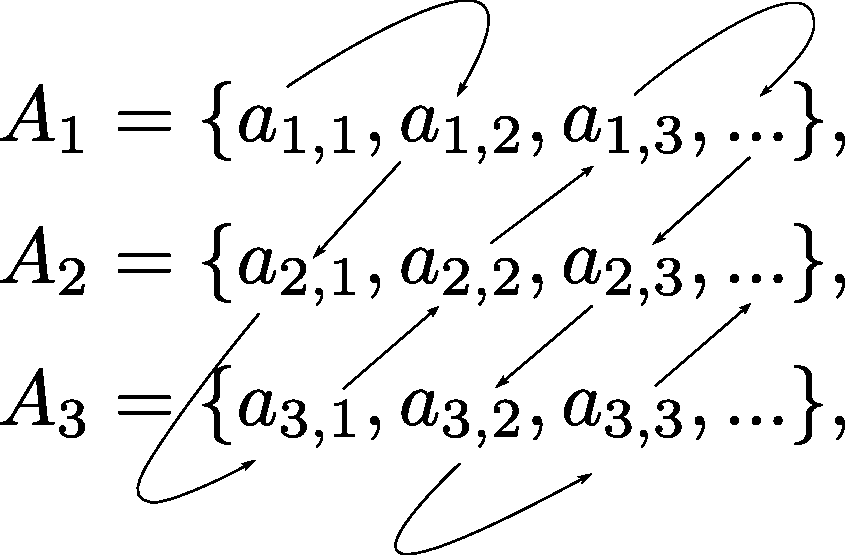
\includegraphics[width=.43\linewidth]{figures/diagonlization.pdf}

\end{center}
    
Which produces a sequence $$A_{n,m}=\{a_{1,1},a_{1,2},a_{2,1},a_{3,1},...\}$$
and so on. Hence, $\bigcup_{\alpha\in J}A_\alpha$ is countable.
\end{proof}

\begin{definition}
	Given a set $A$, the \emph{power set} of $A$, denoted $\mathcal{P}(A)$ or $2^A$, is the set of all subsets of $A$.
\end{definition}
It is a standard combinatorial fact that the cardinality of $2^A$ is equal to $2^{k}$, for $|A|=k$.

\begin{eg}
	Let $A=\{a_1,a_2,a_3\}$. Let $D=\{a_1,a_3\}$ and $E=\{a_2\}$, both subsets of $A$. Then we can define a mapping such that each subset is given by a binary value:

$$A=\{a_1,a_2,a_3\}$$
$$D\mapsto(1,0,1)$$
$$E\mapsto(0,1,0)$$
$$\emptyset\mapsto(0,0,0)$$

and so on.
    
\end{eg}

This idea is essential to the following theorem:

\begin{theorem}
	\emph{Cantor's Theorem} For any set $A$, we have $A \not\sim 2^A$.
\end{theorem}
\begin{proof}
	Suppose that there exists a bijection $f:A\hookrightarrow 2^A$; then $a\mapsto f(a)\subset A$. Then we desire to construct a subset $B\subset A$ such that $B\not\in f(A)$. In particular, let us say that $$B=\{a:a\not\in f(a)\}.$$
    But if $b\in B$, we have $b\not\in f(b)=B$, a contradiction; then $b\not\in B$. But then $b\not\in f(b)=B$; this implies $b\in B$, yet another contradiction. So $B\neq f(b)$ for any $b\in A$, as desired.
    
\end{proof}

\begin{eg}
	By membership, we have $2^A\sim$ \ $\{f\text{ }| \text{ }f:A\rightarrow \{0,1\}$; therefore, there exists a cardinality greater than that of $\R$; namely, the cardinality of $2^\R$.
\end{eg}
The list of cardinalities is $0,1,2,3,4,...,\aleph_0,\aleph_1,\aleph_3,...,\aleph_\alpha,...$ for $\alpha$ an infinite ordinal. Let us say that $|\Z| = \aleph_0$, and that $|\R|=\mathfrak{c}$; the Continuum Hypothesis claims that $\mathfrak{c}=\aleph_1$, a fact which is provably undecidable under ZF+C. 

\begin{definition}
    A set $X$ is a \emph{metric space} if it is endowed with a \emph{metric} $d:X\times X\rightarrow \R$, such that for each $a,b\in X$:
    \begin{enumerate}
        \item $d(a,b)\geq 0$
        \item $d(a,b)=d(b,a)$
        \item \emph{Triangle Inequality} $d(a,b) \leq d(a,r)+d(r,b)$.
    \end{enumerate}
\end{definition}

\begin{eg}
	$\R$ has the standard metric of $d(x,y)=|x-y|$; more generally, $\R^n$ has the Euclidean metric of $$d(\bold{x},\bold{y})=\sqrt{(x_1-y_1)^2+...+(x_n-y_n)^2}.$$
\end{eg}

\begin{eg}
	Let $\R^2$ have the metric $$d(\bold{x},\bold{y})=\sum^n_{i=0}|\bold{x}-\bold{y}|;$$ this would be a completely valid metric on $\R^2$, or even $\R^n$.
\end{eg}

\begin{eg}
	Let us consider the \emph{space of functions}; there are many ways to define a metric on such a space. One way to do so is to define a metric $d$ on the space of continuous functions on the interval $[a,b]$, $\mathcal{C}[a,b]$ :

    $$\int^b_a |f(x)-g(x)|dx.$$
    
\end{eg}

A good way to get a sense for what a metric space is actually \emph{doing} is to use \emph{balls}:

\begin{definition}
	An \emph{open ball} is a set $N_r(x)=\{y:d(x,y)< r\}$. A \emph{closed ball} is a set $\overline{N_r(x)}=\{y:d(x,y)\leq r\}$.
\end{definition}

\begin{definition}
	A \emph{limit point} of a set $E$ is a point $p\in X$ such that every neighborhood of $p$ contains some $p\neq q\in E$.
\end{definition}